\chapter{Molecular Imaging Methods}
\label{sec:imaging}

This chapter introduces two molecular imaging methods,\textit{Computed Tomography} and 
\textit{Cryo-Electron Microscopy} (cryo-EM). 
Further, their observation model is defined in a mathematic way and reconstruction is presented.
Application of cryo-EM is a major motivation for this Thesis, 
as the problem is not easy to solve due to dealing with enormous noise and unknown observation angles.
Moreover, cryo-EM can be seen as a problem in 3D, as original object is in 3D.
CT is similar to cryo-EM, but reconstruction is slightly simpler, since it is potentially in 2D and 
observation angles are known.
That's why it is well suited as a first step towards a cryo-EM algorithm.



\section{Computed tomography}
CT is a well established molecular imaging method.
Using X-ray source, fan shaped beams are produced which scan the imaging object.
Through scanning over straight lines many observations are collected, 
and original object can be reconstructed.\footnote{For further details \cite{computedTomography}}

\paragraph{Tomography reconstruction:}
\textbf{TODO: The aim is to reconstruct a biological sample based on the observation of its projection along  line.}

Tomographic reconstruction is a popular inverse problem. 
The aim is to reconstruct an original object from observations.
When original object is in 2D, observations are available in 1D. 
The reconstruction is possible for 3D objects as well, where observations are in 2D\footnote{For further details \cite{tomographicReconstruction}}.


\begin{tcolorbox}[colback=red!5!white,colframe=red!75!black]
    In this Thesis I focus on the 2D case of CT, which is called \textit{classical tomography }
\end{tcolorbox}

\pagebreak

\paragraph{2D tomographic observation:}

Mathematically, CT observations are defined as follows:

\textbf{TODO:}
\begin{itemize}
    \item equation 3.1, theta in $S^1$, not in R, it's an angle
    \item equation 3.1, R maps into $R^M$, not $L^2$ 
    \item equation 3.1 based on your definition, this would mean that R includes radon transform and discretization operator 
        (should mention it, maybe no need to define it this way)

\end{itemize}

\begin{equation}
    \label{eq:2Dreconstruction}
    \begin{aligned}
        y_i[j] &= p_i + \eta_i[j], & \text{ with } 1 \leq i \leq N \text{ and } 1 \leq j \leq M \\
               &= R(x, \theta_i, s_j) + \eta_i[j], & \text{ with } 1 \leq i \leq N \text{ and } 1 \leq j \leq M
    \end{aligned}
\end{equation}

with
\begin{itemize}
    \item $N$: number of observations
    \item $M$: observation dimension
    \item $y_i \in \mathbb{R}^M$ :  $i$-th observation with $y_i[j] \in \mathbb{R}$: $j$-th element of observation
    \item $p_i \in \mathbb{R}^M$ :  $i$-th noiseless observation with $p_i[j] \in \mathbb{R}$: $j$-th element of noiseless observation
    \item $x \in L^2(\Omega)$ : original object with $\Omega \subset \mathbb{R}^2 $ and $L^2$ Lebesgue space
    \item $R(\cdot; \theta, s): L^2(\Omega) \to L^2(\tilde{\Omega}) , x \mapsto R(x; \theta,s)$ : Radon Transform\footnote{For further details \cite{radonTransform}} 
        with, $\tilde{\Omega} \subset \mathbb{R}$, $\theta_i \in \mathbb{R}$ : observation angle and $s_j \in \mathbb{R}$ : sampling point 
    \item $\eta_i \in \mathbb{R}^M$ : Gaussian noise with $\eta_i[j] \sim \mathcal{N}(0,\sigma^2) \in \mathbb{R}$
\end{itemize}


\paragraph{Observation illustration:}

Output of Radon Transform is called a \textit{sinogram}, which is the CT observation.
In Figure~\ref{fig:phantom} the Shepp-Logan phantom is illustrated.
It is often used as an image for simulating a brain CT and in following refers to original object $x$. 
Further, in Figure~\ref{fig:phantom_sinogram} and Figure~\ref{fig:phantom_sinogram_noisy} 
observation sinograms can be seen with and without noise respectively. 
$\theta$ and $s$ must be defined to apply Radon Transform.
For this example, $\theta \in \mathbb{R}^{500}$ was evenly spaced
between $[0, 2 \pi]$ and $dim(s) = 400$. 
Thus, $p \in \mathbb{R}^{500 \times 400}$ and can be plotted as image with resolution 500x400. 
Further, noise was added to reach an SNR of 10 dB.

\begin{figure}[H]
    \label{fig:phantom_and_sinos}
    % \centering
    \hfill
    \subbottom[\label{fig:phantom}]{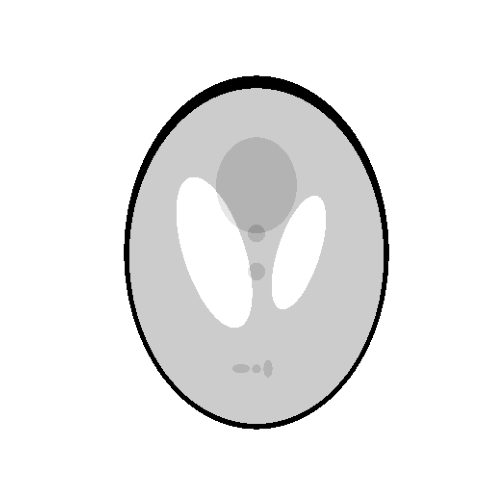
\includegraphics[width=0.3\textwidth]{phantom.png}}
    \hfill
    \subbottom[\label{fig:phantom_sinogram}]{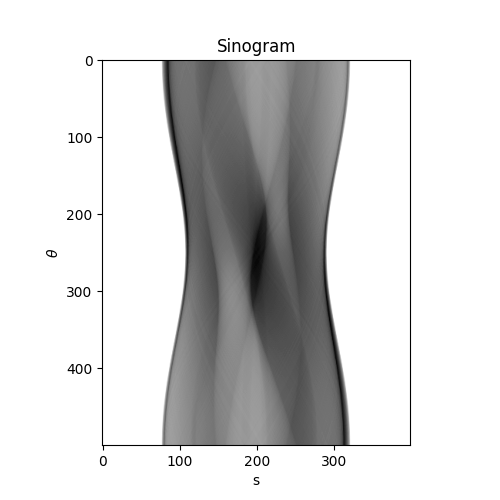
\includegraphics[width=0.3\textwidth]{phantom_sino.png}}
    \hfill
    \subbottom[\label{fig:phantom_sinogram_noisy}]{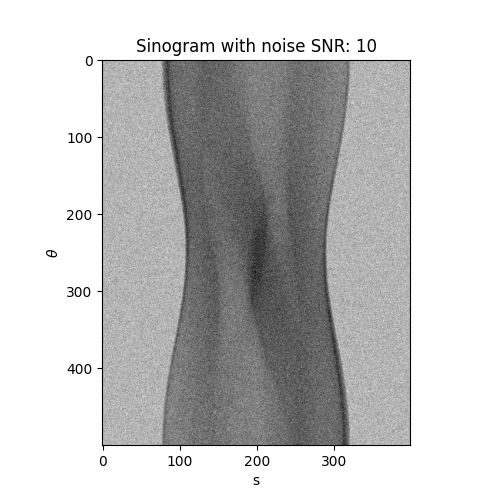
\includegraphics[width=0.3\textwidth]{phantom_sino_noisy_snr10.png}}
    \hfill
	\caption{Shepp-Logan phantom and corresponding sinograms:
    \ref{fig:phantom} Shepp-Logan phantom,
    \ref{fig:phantom_sinogram} clean sinogram: $R(x, \theta, s)$,
    \ref{fig:phantom_sinogram_noisy} noisy sinogram: $R(x, \theta, s) + \eta = y + \eta$ 
    }
\end{figure}

\paragraph{Filter Backprojection:}
\textbf{TODO: FBP, maybe with adding that it is the historical approaches, it has been years during decades. T
hen for a long time people try to improve the results by solving more sophisticated problems using regularisation. 
And recently, Learning has allows a significant increase in the resolution by processing the output of FBP, which is now state of the art. 
And we will use this as reconstruction
}
Filter Backprojection (FBP)~\cite{tomographicReconstruction}, 
is a reconstruction method used in classical tomography.
It allows to inverse the Radon Transform and enables reconstruction of the original object $x$.
It can be defined as:

\begin{equation}
    \label{eq:fbp}
    \textit{FBP}(\cdot; \theta, s) : L^2(\tilde{\Omega}) \to L^2(\Omega), y \mapsto \textit{FBP}(y; \theta, s)
\end{equation}

Where $\theta$ are the projection angles and $s$ are the sampling points.
The algorithm fails when working with noisy data~\cite{cryoEmMath2}, as it is not possible to draw meaningful connections anymore, noise
is dominating information in the data.

\begin{figure}[h]
    \label{fig:phantom_fbps}
    % \centering
    \hfill
    \subbottom[\label{fig:fbp_phantom}]{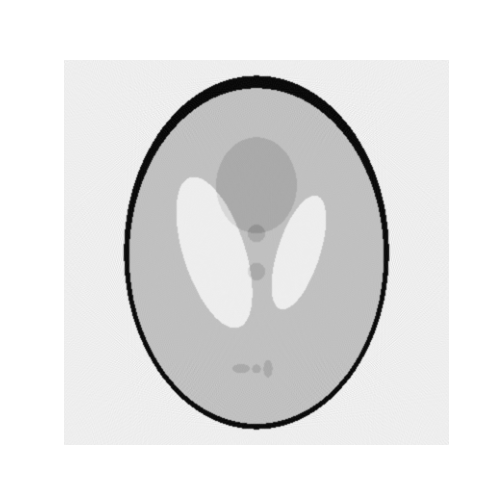
\includegraphics[width=0.3\textwidth]{fbp_phantom_clean.png}}
    \hfill
    \subbottom[\label{fig:fbp_phantom_noisy}]{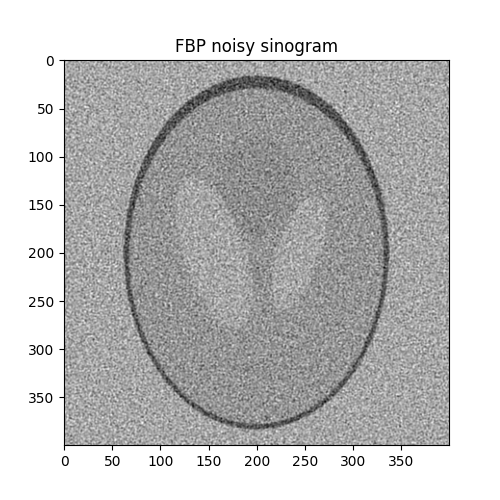
\includegraphics[width=0.3\textwidth]{fbp_phantom_snr_10.png}}
    \hfill
    \subbottom[\label{fig:fbp_unet_phantom_noisy}]{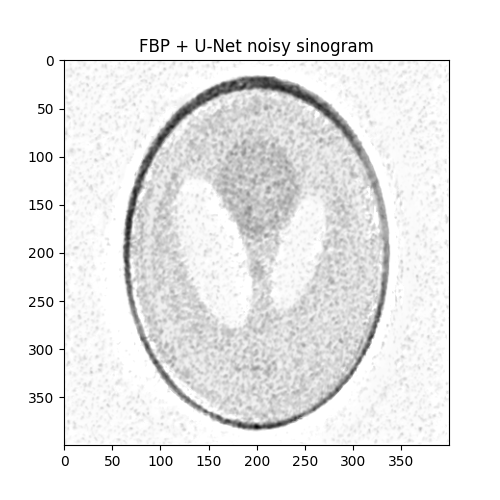
\includegraphics[width=0.3\textwidth]{fbp_unet_phantom_snr_10.png}}
    \hfill
	\caption{Shepp-Logan FBP reconstructions:
    \ref{fig:fbp_phantom} clean reconstruction: $\textit{FBP}(p, \theta, s)$,
    \ref{fig:fbp_phantom_noisy} noisy reconstruction: $\textit{FBP}(y, \theta, s)$,
    \ref{fig:fbp_unet_phantom_noisy} noisy reconstruction: $\textit{UNet}(\textit{FBP}(y, \theta, s))$ 
    }
\end{figure}

Figure~\ref{fig:fbp_phantom} shows reconstruction with clean sinogram, where Figure~\ref{fig:fbp_phantom_noisy} shows
reconstruction from noisy sinogram
The quality of noisy reconstruction is rather low, some important details are missing, and the noise dominates reconstruction.
If more noise is present in $y$, reconstruction will be of even lower quality.

\paragraph{U-Net}

\textbf{TODO:  Unet doesn't seem to crash the problem, it is only slightly better}

\citet{ct-reconstruction-comparison} compared different reconstruction methods for CT. 
Today's state-of-the-art reconstruction algorithms are Deep-Learning based.
U-Net~\cite{unet-tomography}, a convolution neural network approach, performed
much better than only applying FBP, especially when dealing with noise. Figure~\ref{fig:fbp_unet_phantom_noisy} 
shows reconstruction with U-Net where overall noise is drastically decreased.
Additional information about U-Net will follow later in the report.

\section{Cryo-EM}
Cryo-EM is another molecular imaging method, that enables the view of molecules in near-atomic resolution.
In this Thesis, for simplicity, only single-particle cryo-EM~\cite{singleParticleCryoEm} is considered.
When writing about cryo-EM it always refers to single-particle cryo-EM.

During imaging process molecules are frozen in a thin layer of ice, where they are randomly oriented and positioned. 
Random orientation and positioning makes reconstruction challenging, 
but freezing allows observation in a stable state where molecules are not moving.
With an electron microscope, 2D tomographic projection images of molecules are observed,
which are called \textit{micrograph}. 
Frozen molecules are fragile and electron microscope needs to work with
very low power (electron dose), resulting in highly noisy observations. The resulting SNR
is typically smaller than 0 dB, which indicates that there is more noise than signal \cite{cryoEmMath2}.

In addition, observed molecules are not equal in the sense that there are some structural varieties between
molecules (isotopes). While observing the same molecule in ice many times, single observations could be from different isotopes.

\textbf{TODO:  you speak about isotopes and variety, why not (see remark about discussion/conclusion), you should include the keywords conformation here.}


\paragraph{3D cryo-EM reconstruction:}
Cryo-EM reconstruction is defined as estimation of a 3D object from 2D observations.
It can be seen as a 3D problem as the original object $x \in L^2(\Omega)$ to be reconstructed is in 3D.
Based on many observed micrographs the original object $x$ is estimated.
Cryo-EM reconstruction is computational intensive and multiple steps are needed to get from 
observations to the final structure \footnote{for further details \cite{singleParticleCryoEm, cryoEmMath}}.


\textbf{TODO: some inconsistency with M and the number of observation. 
I think Delta should be Omega power M , and then indices (j,k) are taken from Delta.}

\paragraph{3D cryo-EM observation:}
Mathematically, observation is defined as follows:
\begin{equation}
    \label{eq:cryoEmSimple}
    \begin{aligned}
        y_i &= p_i + \eta_i, &\text{ with } 1 \leq i \leq N,\\
        y_i &= \Pi_z  (\; Rot (\;x; \theta_i )) + \eta_i, &\text{ with } 1 \leq i \leq N,    
    \end{aligned}
\end{equation}

where 
\begin{itemize}
    \item $N$: number of observations
    \item $M$: observation dimension
    \item $y_i \in \mathbb{R}^M$:  $i$-th observation with $y_i[j] \in \mathbb{R}$: $j$-th element of observation
    \item $p_i \in \mathbb{R}^M$:  $i$-th noiseless observation with $p_i[j] \in \mathbb{R}$: $j$-th element of observation
    \item $x \in L^2(\Omega)$: original object with $\Omega \subset \mathbb{R}^3 $ and $L^2$: Lebesgue space
    \item $\Pi_z : L^2(\Omega) \to L^2(\tilde{\Omega}), x \mapsto  \int x(\cdot,\cdot,z) dz$: z-axis projection operator,
          with $\tilde{\Omega} \subset \mathbb{R}^2$
    \item $\theta_i = [\theta_i^{(1)}, \theta_i^{(2)}, \theta_i^{(3)} ] $: 3D rotation matrix with $ \theta_i^{(1)}, \theta_i^{(2)}, \theta_i^{(3)} \in \mathbb{R}$ and \\
          $R_{\theta_i} =  R_{e_x} (\theta_i^{(1)}) R_{e_y} (\theta_i^{(2)}) R_{e_z} (\theta_i^{(3)}) = [R^1_{\theta_i}, R^2_{\theta_i}, R^3_{\theta_i}] \in SO(3)$ 
          \footnote{(for further details see \ref{app:3DrotationMatrix})}
          
    \item $\textit{Rot} : L^2(\Omega) \to L^2(\Omega), \textit{Rot}(x, \theta_i) = \left((x_1,x_2,x_3) \mapsto x( x_1R^1_{\theta_i}, x_2R^2_{\theta_i}, x_3R^3_{\theta_i})\right)$: rotation operator
    \item $\eta_i \in \mathbb{R}^M$: Gaussian noise with $\eta_i[j] \sim \mathcal{N}(0,\sigma^2) \in \mathbb{R}$
\end{itemize}

% $y_i \in \mathbb{R}^M$ with $M$ as observation dimension.

% Then, $\Pi_z : L^2(\Omega) \to L^2(\tilde{\Omega}), x \mapsto  \int x(\cdot,\cdot,z) dz$ is projection operator from z-axis
% and $Rot : L^2(\Omega) \to L^2(\Omega), Rot(x, \theta_i) = \left((x_1,x_2,x_3) \mapsto x( x_1R^1_{\theta_i}, x_2R^2_{\theta_i}, x_3R^3_{\theta_i})\right)$ is rotation operator modelling the rotation during freezing.
% Further, $\theta_i = [\theta_i^{(1)}, \theta_i^{(2)}, \theta_i^{(3)} ] $ where entries $ \theta_i^{(1)}, \theta_i^{(2)}, \theta_i^{(3)} \in \mathbb{R}$ and 
% $R_{\theta_i} =  R_{e_x} (\theta_i^{(1)}) R_{e_y} (\theta_i^{(2)}) R_{e_z} (\theta_i^{(3)}) = [R^1_{\theta_i}, R^2_{\theta_i}, R^3_{\theta_i}] \in SO(3)$ is the 3D rotation matrix 
% (see \ref{app:3DrotationMatrix} for further details). 
% $\eta_i \sim \mathcal{N}(0,\sigma^2I) \in \mathbb{R}^M$ corresponds to noise of observation.


As $y_i$ is not observable directly, discretization is needed:
\begin{equation}
    \label{eq:cryoEmSimpleDiscrete}
    \begin{aligned}
        y_i &= \left( \Pi_z (\; Rot (\;x; \theta_i)) + \eta_i\right)(\Delta) &, \text{ with } 1 \leq i \leq N \\
        y_i[j,k] &= \Pi_z (\; Rot(\;x; \theta_i))_{j,k} + \eta_i[j,k] &, \text{ with } 1 \leq i \leq N \text{ and } 1 \leq j,k \leq M
    \end{aligned}
\end{equation}

with
\begin{itemize}
    \item $\Delta \subset \tilde{\Omega}^{M^2}$: sampling grid with dimension $M^2$
    \item $y[j,k]$, $\eta[j,k]$ and $\Pi_z(\cdot)_{j,k}$ $ \in \mathbb{R}$ with $j,k$ as indices of the sampling grid.
\end{itemize}
% $\Delta \subset \tilde{\Omega}^{M^2}$ is the sampling grid with dimension $M^2$.
% Further, $y[j,k]$, $\eta[j,k]$ and $\Pi_z(\cdot)_{j,k}$ $ \in \mathbb{R}$ with $j,k$ as indices of 
% the sampling grid.


\begin{figure}[H]
    \label{fig:cryo-em-omicron}
    % \centering
    \hfill
    \subbottom[\label{fig:omicron}]{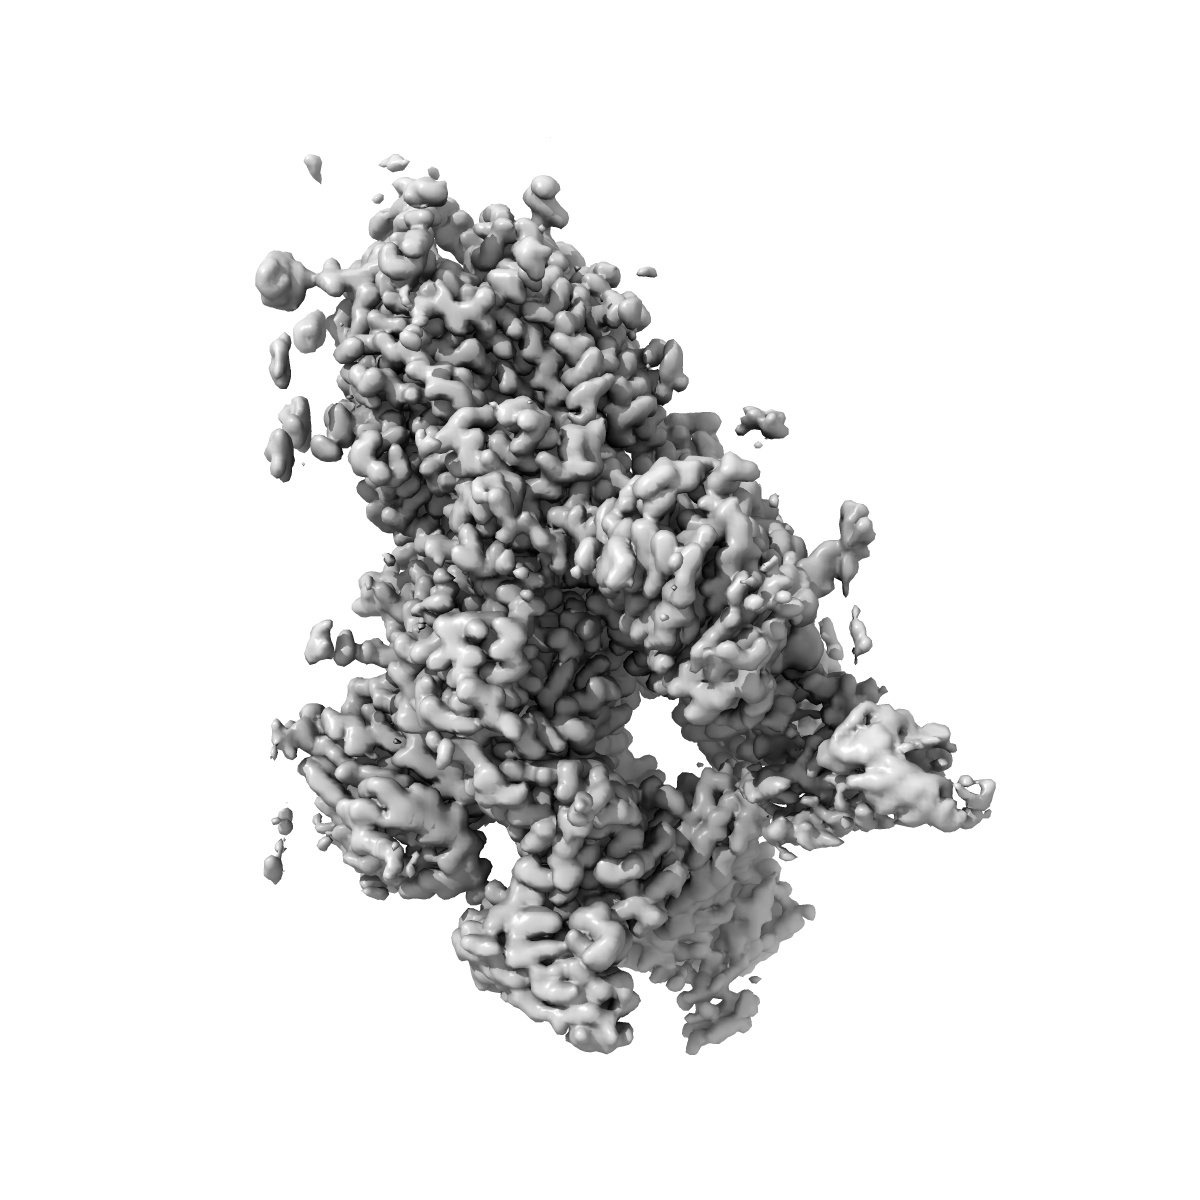
\includegraphics[width=0.18\textwidth]{emd_32500.map_xsurface.jpeg}}
    \hfill
    \subbottom[\label{fig:omicron-x}]{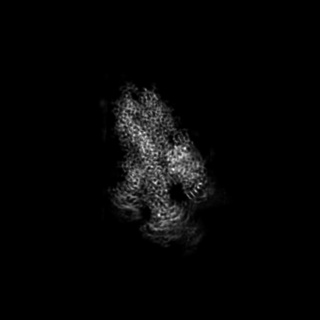
\includegraphics[width=0.18\textwidth]{emd_32500.map_xprojection.jpeg}}
    \hfill
    \subbottom[\label{fig:omicron-y}]{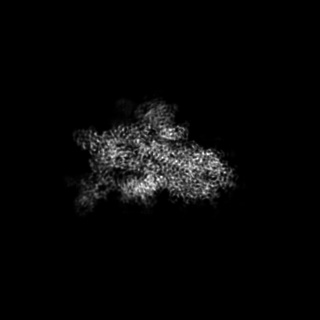
\includegraphics[width=0.18\textwidth]{emd_32500.map_yprojection.jpeg}}
    \hfill
    \subbottom[\label{fig:omicron-z}]{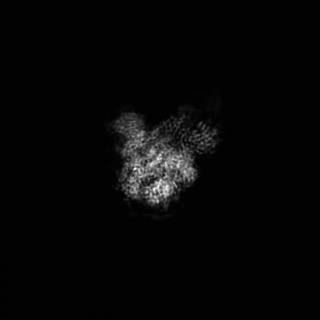
\includegraphics[width=0.18\textwidth]{emd_32500.map_zprojection.jpeg}}
    \hfill
	\caption{Cryo-EM reconstruction and clean projections of COVID-19 Omicron spike \protect\footnote{https://www.ebi.ac.uk/emdb/EMD-32500}: 
    \ref{fig:omicron} COVID-19 Omicron spike,
    \ref{fig:omicron-x} projection along x-axis,
    \ref{fig:omicron-y} projection along y-axis,
    \ref{fig:omicron-z} projection along z-axis
    }
\end{figure}


\paragraph{Extended formula:} 
\textbf{TODO: not sure what this mean. 
Maybe "more realistic modeling" .
 ou could have a remark about variety of molecule (once for all, and say we don't consider it), a remark about the psf 
 }

Equation~\ref{eq:cryoEmSimple} is a simplified version of cryo-EM.
First, point spread function (PSF) of the microscope is not taken into account.
Second, structural variety is ignored, the underlying object $x$ is not the same 
for every observation. 
Precisely, $x$ can be seen as a random signal from an unknown distribution defined over all possible molecules structures.

Equation~\ref{eq:cryoEmSimple} can be extended and defined as the following:
\begin{equation}
    \label{eq:cryoEmExtended}
    \begin{aligned}
        y_i = h_i \star \Pi_z ( \textit{Rot} (x_i; \theta_i)) + \eta_i &, \text{ with } 1 \leq i \leq N    
    \end{aligned}
\end{equation}

Where $h_i$ is the PSF of the microscope and $\star$ defines convolution.
Further, $x_i \in X$ where $X$ is the set of all possible molecule structures.


\paragraph{Difference to tomographic reconstruction:}
The problems are highly related, but cryo-EM reconstruction is more challenging.
During CT observation, the patient is asked to not move and therefore, angles of projections are known.
Whereas, in cryo-EM, this information will be lost during freezing.
Second, high level of noise makes cryo-EM much more challenging.

\clearpage

\section{Abstraction}

\textbf{TODO:  you can say that we do that to motivate the fact that 2d and 3d are mathematically very similar,
and that extended numerical procedure from 2d 
(as done in the thesis) to 3d should be theoretically feasible, it remains only numerical questions due to, 
of course, an extra need in resources}

\label{sec:abstract_form}
As tomographic reconstruction and cryo-EM reconstruction are similar, 
goal of this Thesis is to design an algorithm, that can be applied in both scenarios.

Therefore, an abstract form of the problems will be defined.
A similar notation than previously is used, with original object $x \in L^2(\Omega)$.
Further, original object dimension space is parametrized with $D$, consequently $\Omega \subset \mathbb{R}^D$.
Additionally, dimension of observation space is defined as $D-1$, such that 
$\tilde{\Omega} \subset \mathbb{R}^{D-1}$.


\begin{equation}
    \label{eq:abstract-model}
    \begin{aligned}
        y_i &= p_i + \eta_i (\Delta) &, \text{ with } 1 \leq i \leq N \\
        y_i &= \left( A(x, \theta_i) + \eta_i \right) (\Delta) &, \text{ with } 1 \leq i \leq N 
    \end{aligned}
\end{equation}
with
\begin{itemize}
    \item $N$: number of observations
    \item $M$: observation dimension
    \item $y_i \in \tilde{\Omega}^M$: the $i$-th observation
    \item $p_i \in \tilde{\Omega}^M$: the $i$-th noiseless observation
    \item $x \in L^2(\Omega)$: original object
    \item $A: L^2(\Omega) \to L^2(\tilde{\Omega}), x \mapsto A(x; \theta_i)$: a non-linear operator 
    \item $\theta_i \in \mathbb{R}^P$: projection angle(s) vector, with $P$ projection dimension
    \item $\eta \sim \mathcal{N}(0, \sigma^2 I) \in \tilde{\Omega}^M$: Gaussian noise
    \item $\Delta \subset \tilde{\Omega}^{M}$: term for discretization
\end{itemize}

\paragraph{Reconstruction:}
\textbf{TODO: 
equation 3.7, Delta is Omega tilde power M not power D.
Also, as before, theta is in SO(3) (in equation 3.3 also theta should be in [0,2pi], maybe with finding a consistent definition)}


Further, an abstract form of the reconstruction operator is defined as:

\begin{equation}
    \textit{Recon} : L^2(\tilde{\Omega}) \to L^2(\Omega), y \mapsto Recon(y; \theta)
\end{equation}

with
\begin{itemize}
    \item $\theta_i \in \mathbb{R}^P$: projection angle(s) vector, with $P$ projection dimension
\end{itemize}

\textbf{Check: Theta and discretization term}

\paragraph{Classical tomography:}

Classical tomography parameters are defined with $D=2$, $P=1$.
Further, $A(\cdot)$ is the Radon Transform (see Equation~\ref{eq:2Dreconstruction}).
Reconstruction operator can be defined as FBP (with or without U-Net).

\paragraph{Cryo-EM:}
Cryo-EM parameters are defined with $D=3$ and $P=3$ as $\theta_i$ not only corresponds to
a projection angle vector but also some rotation.
Further, $A(\cdot)$ can be defined as $\Pi_z \left(\; \textit{Rot}(\;x; \theta) \right)$ 
where \textit{Rot} is the 3D rotation and $\Pi_z$ the tomographic projection.

\paragraph{High noise regime:}
Cryo-EM observations are highly noisy, which makes reconstruction challenging. 
There are different ways to reduce noise from observations, most of them are related to averaging. 
Averaging needs to consider similar observations and ignore diverse ones. 
In the defined abstract model, averaging over paired observations from $\theta$ should be a good averaging model.

One idea would be to measure distances between observations.
Another way is to find a low-dimensional embedding which maps observation $y$ to $\theta$.
When talking from low-dimensional embeddings, there is no way around Graph Learning, which will be introduced
in the following Chapter~\ref{sec:graphFoundations} \textit{\nameref{sec:graphFoundations}}.
